\chapter{Project Management}
\label{ch:projman}

In this chapter we discuss and evaluate the methodology and tools used to undertake the project.

\section{Methodology}
The project is very practical, with much of the time spent writing and testing HDL code. As such, an appropriate engineering methodology is employed. Figure \ref{fig:methodology} gives an overview of our development process and design flow.

Our high-level approach is very plan based: we start with the design outlined in Chapter \ref{ch:design}, detailing the instruction set and then block design of the PIO device, defining all the HDL modules needed and the relationships and connections between them. Having a detailed design on paper before any code is written is advantageous in many aspects: the design is well documented, and allows to focus on the implementation details of each module while writing code instead of worrying about higher level architectural details.

Implementation begins with taking the block design in Chapter \ref{ch:design}, and building it out into a skeleton Scala project with all the Chisel modules required as detailed in Chapter \ref{ch:implementation}. Once this structure is in place, we implement the modules one at a time, writing and testing code in an iterative fashion. Any issues identified in the design during implementation were first fixed in the block design or instruction set, and then propagated through the entire design process from there, fixing any problems as we followed the design flow through.

On a high level this is a very structured, plan-based methodology. It borrows from the waterfall methodology: first defining requirements and objectives, laying out a detailed design, and then implementing based on the design. Going back to the start and following back through the design process when any changes need to be made is another trait borrowed from the waterfall methodology \cite{softeng}. This kind of methodology is ideal for a project such as ours that is both complex and needs to be well documented.

Where this methodology differs from waterfall is when it comes to the implementation on a per-module level. Instead of writing all the code before moving on to the testing phase (as in a traditional waterfall style), each module was written and tested before moving on to the next. The module interfaces and requirements were already well-defined, so development on a module level was a case of working with chisel to implement the required logic. This ended up being quite an experimental and iterative process, due in part to the author's inexperience with Chisel. More time during the earlier design stages to lay out implementation details for each module would perhaps have been time well spent, as it would have enabled a more methodical approach to development, and reduced the amount of time spent experimenting within Chisel.

This approach leans into a much more agile style of development, borrowing ideas of incremental development and constant testing from extreme programming methodologies. This is a very natural style of development team of only one person, and easy when there are no external stakeholders or customers required to validate the incremental product \cite{softeng}.

The testing process is also inspired by agile methodologies. Test-driven development is used heavily, writing unit tests for each module alongside the module itself, with the implementation and functional verification processes interleaved. Chisel's close integration with it's testing and verification tools (ChiselTest \& Treadle, as mentioned in Chapter \ref{ch:evaluation}) makes it easy to rapidly write testbenches. The codebase includes a large test suite as a result of this, which allowed to develop and iterate quickly and with confidence.

End-to-end system-level verification also takes place: verifying that the design synthesises correctly, and testing the system in simulation and with software as outlined in Chapter \ref{ch:evaluation}. This system validation process rounds off the waterfall methodology we employ.

Overall this methodology worked very well, and was well-suited to the nature of the project. However, towards the end it became evident that more flexibility was needed when it came to end-to-end and system testing: issues identified during system testing took a long time to fix, as it involved going back through the full design flow. This issue was exacerbated by the long FPGA synthesis times and complexity of configuring the synthesis process for debugging. A plan to better iterate between the design and system testing would have allowed to faster fix bugs, and allowed for more time to run simulations and develop test software towards the end of the project.


\begin{figure}[H]
    \centering
    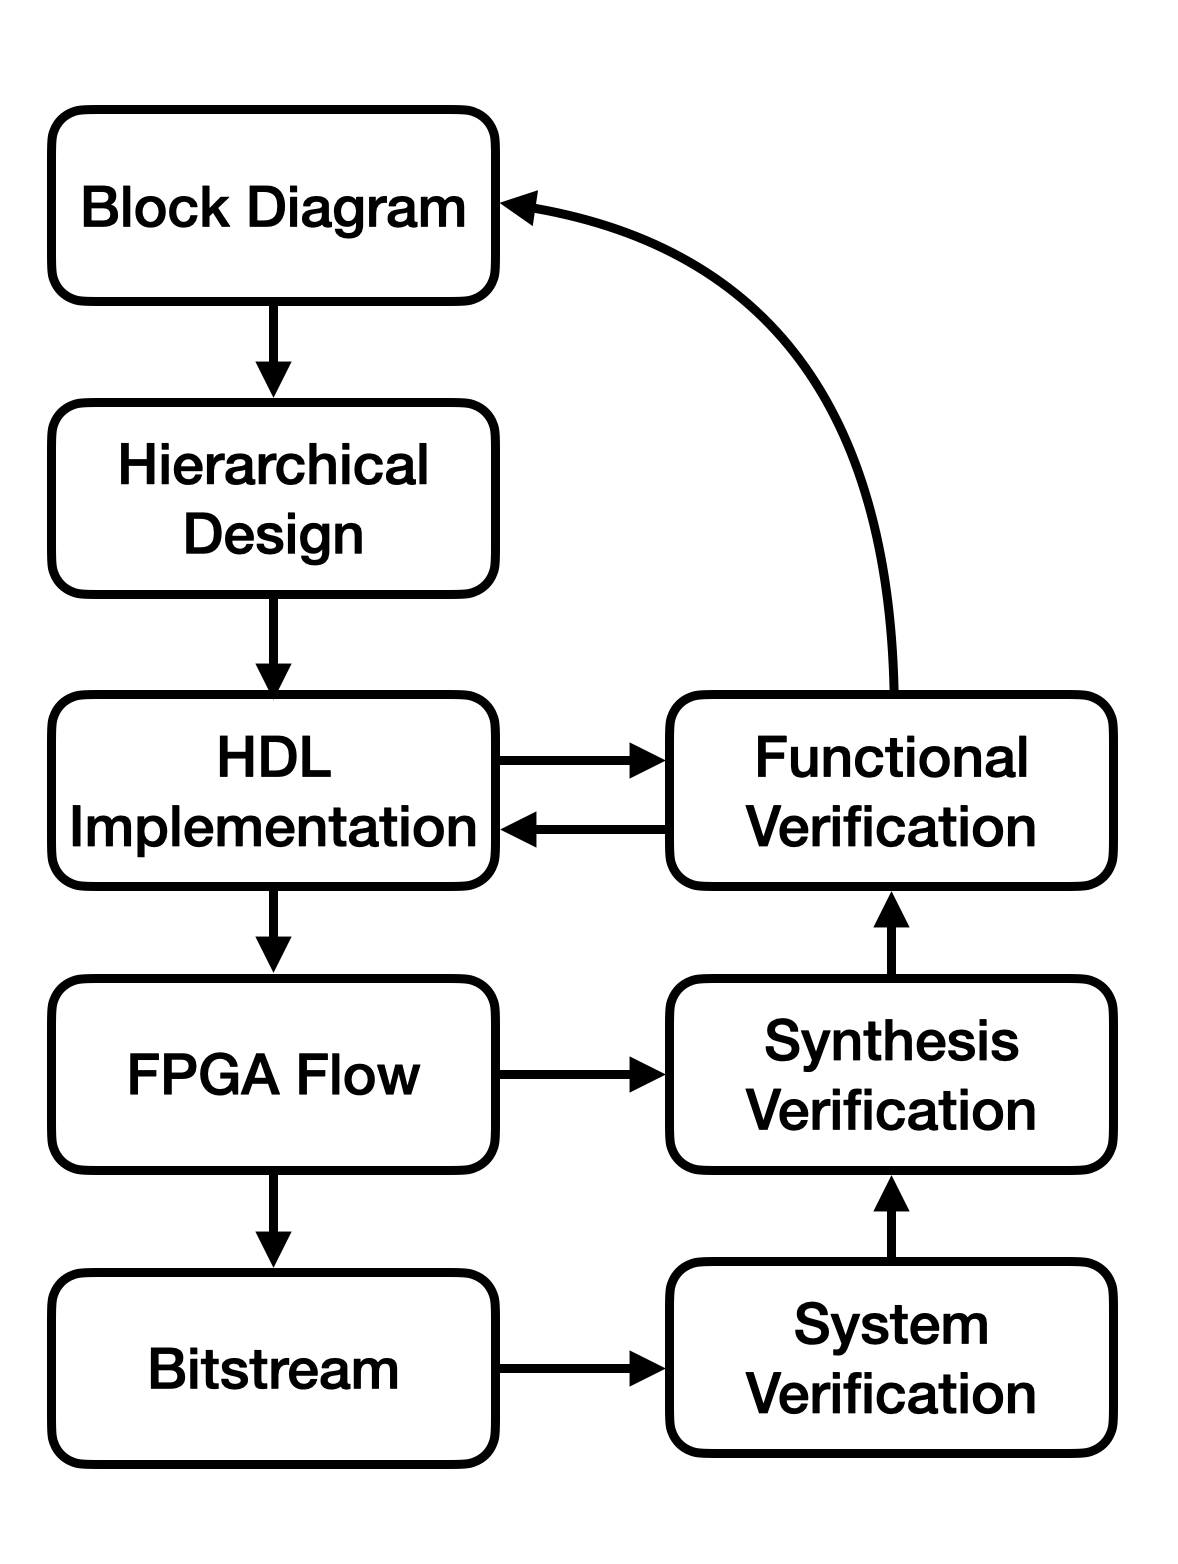
\includegraphics[width=0.6\textwidth]{../img/methodology.png}
    \caption{An overview of our development methodology}
    \label{fig:methodology}
\end{figure}


\section{Timeline}
The project commenced at the start of October 2022 (Week 1) with the submission of the project specification. The timeline as stated in the specification (Timeline A) is given in Table \ref{tab:timeline}, along with the timeline as revised at the end of November 2022 (Week 9) (Timeline B), and the actual timeline which the project followed (Timeline C).

\begin{table}[ht!]
    \centering
    \begin{tabular}{|p{0.52\textwidth}|p{0.12\textwidth}|p{0.12\textwidth}|p{0.12\textwidth}|}
        \hline
        \multirow{2}{*}{\textbf{Task}}                                      & \multicolumn{3}{c|}{\textbf{Week(s)}}                                             \\ \cline{2-4}
                                                                            & \textbf{Timeline A}                   & \textbf{Timeline B} & \textbf{Timeline C} \\ \hline
        Background research                                                 & 1-2                                   & 1-4                 & 1-4                 \\ \hline
        Implement proof of concept I/O device in Chisel                     & 3-5                                   & 4-11                & 4-11                \\ \hline
        Lay out high-level block design                                     & 6-8                                   & 12                  & 12-13               \\ \hline
        Extend proof of concept into project skeleton based on block design & 8-11                                  & 13                  & 14                  \\ \hline
        Write HDL code, implementing and testing one module at a time       & 12-18                                 & 14-19               & 15-19               \\ \hline
        Develop and run integration tests in simulation                     & 19                                    & 20                  & 20-23               \\ \hline
        Use Rocket Chip to integrate device with RISC-V cores               & 20-21                                 & 21-22               & 21                  \\ \hline
        Load microcontroller onto FPGA and run tests                        & 22-24                                 & 23-24               & 22-23               \\ \hline
        Write report                                                        & 25-31                                 & 25-31               & 24-31               \\ \hline
    \end{tabular}
    \caption{Project Timeline}
    \label{tab:timeline}
\end{table}

Very little project work took place in the first 10 weeks, due to more time being consumed by other modules and coursework. More time was also spent getting to grips with Chisel and Scala than anticipated, figuring out effective workflows for integrating Chisel and it's compilation process into Vivado's design flow while developing a very basic proof-of-concept. This was not an entirely unforeseen problem as we were working with unfamiliar technologies, and could have been better accounted for this in the original timeline. Despite this eating into the early stages of the project, the time was not felt to be wasted, as it gave a strong foundation on which to build during development.

After week 13 when the block design was complete, the original timeline was mostly caught up to and proceeded as planned. Development was completed by week 19, when effort shifted to system verification both in simulation and with software. The Rocket chip integration process, simulation and system verification processes also ended up becoming more interleaved towards the end of the project, as lots of time was spent debugging and iterating back through the design process. The timeline was cut short by a week due to the need to present results as part of the project presentation at the end of week 23. As a result of this, there was less time to run tests on the FPGA and the test software only demonstrated very basic capabilities.

The timeline and associated tasks were tracked using an interactive Kanban board\footnote{\url{https://github.com/users/Joeyh021/projects/2/}} as part of GitHub's project features. Each of the tasks listed in Table \ref{tab:timeline}, as well as any other tasks that came up, were added to the board and categorised as either `Todo', `In Progress', `Completed' or `Blocked'. Comments were left on each task to keep notes on progress, and reference specific Git commits or code associated with the tasks. This was valuable for keeping track of progress, especially as work ramped up and multiple tasks were being worked on towards the end of the project. This was something that could have been better kept on top of and better utilised, which may have resulted in a better and more coherently managed project on a day-to-day basis.

\section{Tools \& Resources}

A number of software tools and hardware resources were utilised to make this project possible and assist with development.

\subsection{Source Control}

Code was tracked using Git, the industry standard tool for source code management and version control \cite{git}. All code was committed to a single repository, with commits kept atomic and incremental to best keep track of the repository's version history. Multiple branches were used when experimenting with different ideas, which facilitated easily switching back and forth between different prototypes. Being able to move around between different versions of the code and easily revert changes was very valuable.

For remote backup of source code, GitHub was used. GitHub provides remote Git repositories which local repositories can push and pull from, allowing for convenient remote syncing \cite{github}. This was also convenient for working accross multiple machines, as work was always pushed to the remote repository and new commits could be pulled down from the remote.

GitHub includes GitHub Actions, a continuous integration and deployment platform (CI/CD) that allows to automatically run tests (and other things) when code is pushed to a remote repository  \cite{gha}. GitHub Actions was configured to run all the full suit of unit tests every time a new commit was pushed, which helped to detect regressions in the code where changes had caused bugs that had gone unnoticed, with any failures causing a notification to be sent to the authors.

\subsection{Scala \& Chisel}

The Chisel compiler and standard library are provided as a set of libraries for Scala, so ultimately the Chisel compilation process requires both a Scala compiler to compile the Scala source to Java bytecode, and a Java Virtual Machine on which to run.

The Scala 2 compiler, scalac (distinct from the Scala 3 compiler, dotty), is available on GitHub under the open source Apache License 2.0. This was utilised in combination with sbt, a Scala build tool (sbt is not an acronym for Scala Build Tool) to manage builds and external dependencies. sbt is also avaible on GitHub under the same open source license. sbt was especially useful as it abstracts away the complexity of compiling all of the code and libraries into a single \txt{sbt build} command.

The Chisel libraries were included in the project via definitions in sbt's \txt{build.sbt} file, which allows sbt to then automatically fetch the library packages from Maven Central, where the compiled library artifacts are published for use \footnote{\url{https://mvnrepository.com/artifact/edu.berkeley.cs/chisel3}}. Chisel's source code is also published on GitHub under the Apache License 2.0.

sbt did cause some issues during the course of the project due to the complexity of it's DSL for the \txt{build.sbt} file, and due to idiosyncrasies in it's dependency resolution. Alternative build tools were not explored due to sbt's ubiquity, but evaluating the use of an alternaive such as Mill \cite{Mill} or Gradle \footnote{\url{https://gradle.org/}} may have made managing builds smoother.

Open source JDK builds \footnote{\url{https://openjdk.org/}} were used, both on Linux and MacOS.

\subsection{FPGA Tools}

To synthesise Verilog and generate bitstreams for the FPGA, Xilinx's Vivado design suite and toolchain was used. Xilinx FPGA bitstream formats are entirely propietary, and Vivado is also propietary software. A free version with limited functionality is made available under strict licensing terms. Vivado was utilised primarily on the author's personal Ubuntu workstation PC. The Digilent Nexys A7-100T FPGA board utilised was provided by the School of Engineering. The FPGA board had enough logic resources to synthesise the PIO and a full SoC, something which was evaluated early on in the project to establish that the hardware would be suitable.

